%& C:\Users\Dell\AppData\Roaming\TikzEdt\TikzEdt\023~1.0\TEMP_H~1
\begin{document}
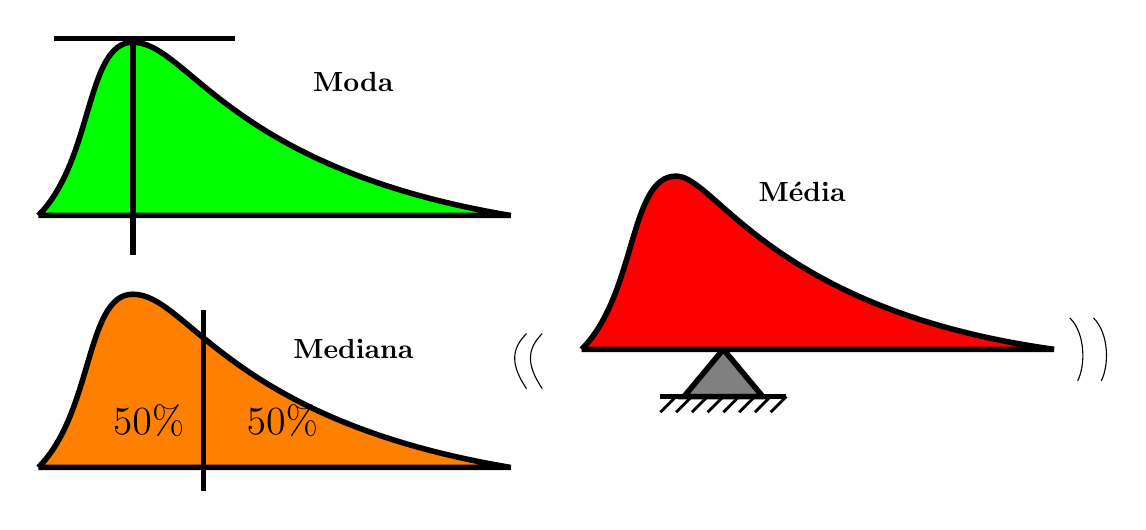
\begin{tikzpicture}
%\node {\includegraphics{ModeMeanMedian.jpeg}};
\draw[line width=2, fill=green] (-4.9,1.7) .. controls (-4.2,2.4) and (-4.3,3.9) .. (-3.7,3.9) .. controls (-3,3.9) and (-2.5,2.3) .. (1.1,1.7) .. controls (-1,1.7) and (-2.1,1.7) .. (-4.9,1.7);
\draw[line width=2] (-4.7,3.95) -- (-2.4,3.95);
\draw[line width=2] (-3.7,3.95) -- (-3.7,1.2);
\node at (-0.9,3.4) {\bf{Moda}};

\draw[line width=2, fill=orange] (-4.9,-1.5) .. controls (-4.2,-0.8) and (-4.3,0.7) .. (-3.7,0.7) .. controls (-3,0.7) and (-2.5,-0.9) .. (1.1,-1.5) .. controls (-1,-1.5) and (-2.1,-1.5) .. (-4.9,-1.5);
%\draw[line width=2] (-4.7,3.95) -- (-2.4,3.95);
\draw[line width=2] (-2.8,0.5) -- (-2.8,-1.8);
\node at (-3.5,-0.9) {\Large \bf{$50\%$}};
\node at (-1.8,-0.9) {\Large \bf{$50\%$}};
\node at (-0.9,0) {\bf{Mediana}};
\draw[line width=2, fill=red] (2,0) .. controls (2.7,0.7) and (2.6,2.2) .. (3.2,2.2) .. controls (3.7,2.2) and (4.4,0.5) .. (8,0) .. controls (5.9,0) and (4.8,0) .. (2,0);
%\draw[line width=2] (-4.7,3.95) -- (-2.4,3.95);
\draw[line width=2] (-3.7,3.95) -- (-3.7,1.2);
\draw[line width=2, fill=gray] (3.8,0) -- (3.3,-0.6) -- (4.3,-0.6) -- (3.8,0);
\draw[line width=2] (3,-0.6) -- (4.6,-0.6);
\draw[line width=1] (3.2,-0.6) -- (3,-0.8);
\draw[line width=1] (3.4,-0.6) -- (3.2,-0.8);
\draw[line width=1] (3.6,-0.6) -- (3.4,-0.8);
\draw[line width=1] (3.8,-0.6) -- (3.6,-0.8);
\draw[line width=1] (4,-0.6) -- (3.8,-0.8);
\draw[line width=1] (4.2,-0.6) -- (4,-0.8);
\draw[line width=1] (4.4,-0.6) -- (4.2,-0.8);
\draw[line width=1] (4.6,-0.6) -- (4.4,-0.8);
\draw (1.5,0.2) .. controls (1.3,0) and (1.3,-0.2) .. (1.5,-0.5);
\draw (1.3,0.2) .. controls (1.1,0) and (1.1,-0.2) .. (1.3,-0.5);
\draw (8.2,0.4) .. controls (8.4,0.2) and (8.4,-0.2) .. (8.3,-0.4);
\draw (8.5,0.4) .. controls (8.7,0.2) and (8.7,-0.2) .. (8.6,-0.4);
\node at (4.8,2) {\bf{Média}};

\usetikzlibrary{calc}
\pgftransformreset
\node[inner sep=0pt,outer sep=0pt,minimum size=0pt,line width=0pt,text width=0pt,text height=0pt] at (current bounding box) {};
%add border to avoid cropping by pdflibnet
\foreach \border in {0.1}
  \useasboundingbox (current bounding box.south west)+(-\border,-\border) rectangle (current bounding box.north east)+(\border,\border);
\newwrite\metadatafile
\immediate\openout\metadatafile=\jobname_BB.txt
\path
  let
    \p1=(current bounding box.south west),
    \p2=(current bounding box.north east)
  in
  node[inner sep=0pt,outer sep=0pt,minimum size=0pt,line width=0pt,text width=0pt,text height=0pt,draw=white] at (current bounding box) {
\immediate\write\metadatafile{\p1,\p2}
};
\immediate\closeout\metadatafile
\end{tikzpicture}

\end{document}
